	\section{Week 3 - Logistic Regression}
	
	\subsection{Logistic Function}
	\begin{itemize}
		\item A logistic function (or logistic curve) is a common sigmoid function, given its name (in reference to its S-shape) in 1844 or 1845 by Pierre François Verhulst who studied it in relation to population growth. 
		
		\item A generalized logistic curve can model the "S-shaped" behaviour (abbreviated S-curve) of growth of some population P. 
		
		\item The initial stage of growth is approximately exponential; then, as saturation begins, the growth slows, and at maturity, growth stops.
		The logistic function is the sigmoid curve with equation:
		\[ f(x) = \frac{1}{1 + \mathrm e^{-x}} \]
		
	\end{itemize}
	
	
\subsection{Question 1}

Suppose that you have trained a logistic regression classifier, and it outputs on a new examplex a prediction $h\theta(x)$ = 0.7.
This means (check all that apply): 
\begin{itemize}
	\item Our estimate for$ \Pr(y|=1|x;\theta)$ is 0.7.
	\item Our estimate for$ \Pr(y|=0|x;\theta)$ is 0.3.
	\item Our estimate for$ \Pr(y|=1|x;\theta)$ is 0.3.
	\item Our estimate for$ \Pr(y|=0|x;\theta)$ is 0.7.
\end{itemize}
%======================================================%
%-----------------------------%


\textbf{Solution} 
\begin{itemize}
\item Our estimate for $ \Pr(y|=1|x;\theta)$ is 0.7.  T
$h\theta(x)$ is precisely$ \Pr(y|=1|x;\theta)$ , so each is 0.7.
\item Our estimate for $ \Pr(y|=0|x;\theta)$ is 0.3.  
T Since we must have $ \Pr(y|=0|x;\theta)$ = 1-$ \Pr(y|=1|x;\theta)$ , the former is 1-0.7=0.3 .
\item Our estimate for $ \Pr(y|=1|x;\theta)$ is 0.3.  
F $h\theta(x)$ gives $ \Pr(y|=1|x;\theta)$ , not 1-$ \Pr(y|=1|x;\theta)$ . 
\item Our estimate for $ \Pr(y|=0|x;\theta)$ is 0.7.  
F $h\theta(x)$ is $ \Pr(y|=1|x;\theta)$ , not $ \Pr(y|=0|x;\theta)$
\end{itemize}
 

%======================================================%

	
	%-------------------------------------------------------------------------%
	\subsection*{Question 2. }
	Suppose you have the following training set, and fit a logistic regression classifier h$\theta$(x) = g($\theta_0$ + $\theta$1$x_1$ + $\theta$2$x_2$).
	
	\begin{figure}[h!]
\centering
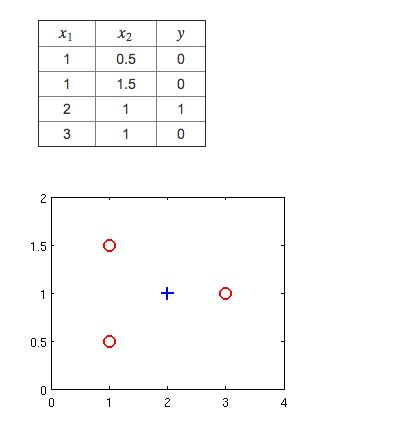
\includegraphics[width=0.6\linewidth]{Week3-Quiz-1}

\end{figure}

	
	Which of the following are true? Check all that apply.
	
	%-------------------------------------------------------------------------%
	\subsection{Question 3. variant
		}
	Suppose you train a logistic classifier h$\theta$(x)=g($\theta$0+$\theta$1x1+$\theta$2x2). 
	Suppose $\theta$0=-6,$\theta$1=0,$\theta$2=1. 
	
	Which of the following figures represents the decision boundary found by your classifier?
	
	%-------------------------------------------------------------------------%
	\subsection*{Question 3. }
	For logistic regression, the gradient is given by EQUATION
	
	%%∂∂$\theta$jJ($\theta$)=1m∑mi=1(h$\theta$(x(i))−y(i))x(i)j. 
	\begin{figure}[h!]
\centering
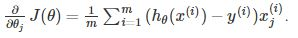
\includegraphics[width=0.5\linewidth]{Week3-Quiz-2}

\end{figure}

	Which of these is a correct gradient descent update for logistic regression with a learning rate of $\alpha$? Check all that apply.

	%-------------------------------------------------------------------------%
	\subsection*{Question 4. }
	Which of the following statements are true? Check all that apply.
	
	\begin{itemize}
\item WRONG J($\theta$) will be a convex function, so gradient descent should converge to the global minimum.

\item CORRECT Adding polynomial features (e.g., instead using h$\theta$(x)=g($\theta$0+$\theta$1x1+$\theta$2x2+$\theta$3x21+$\theta$4x1x2+$\theta$5x22) ) could increase how well we can fit the training data.

\item WRONG The positive and negative examples cannot be separated using a straight line. So, gradient descent will fail to converge.

\item WRONG Because the positive and negative examples cannot be separated using a straight line, linear regression will perform as well as logistic regression on this data.
	\end{itemize}



%======================================================%
%-----------------------------%

\begin{itemize}
	\item Adding polynomial features (e.g., instead using h(x)=g(0+1x1+2x2+3x12+4x1x2+5x22) ) could increase how well we can fit the training data.  
	\item The positive and negative examples cannot be separated using a straight line. So, gradient descent will fail to converge.
	
	\item At the optimal value of $\theta$ (e.g., found by fminunc), we will have $ J(\theta) \geq $0 . 
	\item Because the positive and negative examples cannot be separated using a straight line, linear regression will perform as well as logistic regression on this data.
	solution
\end{itemize}

\subsubsection*{Discussion}
\begin{enumerate}
\item Adding polynomial features (e.g., instead using h(x)=g(0+1x1+2x2+3x12+4x1x2+5x22) ) could increase how well we can fit the training data.  
\begin{framed}
TRUE
Adding new features can only improve the fit on the training set: since setting $\theta_3=\theta_4=\theta_5=0$ makes the hypothesis the same as the original one, gradient descent will use those features (by making the corresponding $\theta_j$ non-zero) only if doing so improves the training set fit. 
\end{framed}
\item 
The positive and negative examples cannot be separated using a straight line. So, gradient descent will fail to converge. 
\begin{framed}
	FALSE
While it is true they cannot be separated, gradient descent will still converge to the optimal fit. Some examples will remain misclassified at the optimum. 
\end{framed}

\item 
At the optimal value of $\theta$ (e.g., found by fminunc), we will have $ J(\theta) \geq$0 . 
\begin{framed}
	TRUE
The cost function $ J(\theta)$ is always non-negative for logistic regression. 
\end{framed}

\item 
Because the positive and negative examples cannot be separated using a straight line, linear regression will perform as well as logistic regression on this data. 
\begin{framed}
	FALSE
While it is true they cannot be separated, logistic regression will outperform linear regression since its cost function focuses on classification, not prediction. 
\end{framed}
\end{enumerate}

%======================================================%
%-----------------------------%








%======================================================%
%-----------------------------%



\subsection{Question 5}
Which of the following statements are true? Check all that apply.

\begin{itemize}
\item For logistic regression, sometimes gradient descent will converge to a local minimum (and fail to find the global minimum). This is the reason we prefer more advanced optimization algorithms such as fminunc (conjugate gradient/BFGS/L-BFGS/etc).

\item Since we train one classifier when there are two classes, we train two classifiers when there are three classes (and we do one-vs-all classification).

\item The sigmoid function g(z) is never greater than one (>1). g(z)=11+e-z

\item 
The one-vs-all technique allows you to use logistic regression for problems in which eachy(i) comes from a fixed, discrete set of values.
\end{itemize}


%======================================================%




\textbf{Solutions}
\begin{enumerate}
\item For logistic regression, sometimes gradient descent will converge to a local minimum (and fail to find the global minimum). This is the reason we prefer more advanced optimization algorithms such as fminunc (conjugate gradient/BFGS/L-BFGS/etc).  0.00

The cost function for logistic regression is convex, so gradient descent will always converge to the global minimum. We still might use a more advanded optimization algorithm since they can be faster and don't require you to select a learning rate. 

\item
Since we train one classifier when there are two classes, we train two classifiers when there are three classes (and we do one-vs-all classification).  

We need to train three classifiers if there are three classes; each one treats one of the three classes as the y=1 examples and the rest as the y=0 examples. 

\item
The sigmoid function g(z) is never greater than one (>1).   

The denominator ranges from  to1 asz grows, so the result is always in(0,1) . 
\item
The one-vs-all technique allows you to use logistic regression for problems in which each y(i) comes from a fixed, discrete set of values. 
If each y(i) is one of k different values, we can give a label to each $y(i)\in\{1,2,\ldots,k\}$ and use one-vs-all as described in the lecture. 

\end{enumerate}










%---------------------------------------------------------------------------%

%---------------------------------------------------------------------------%

%---------------------------------------------------------------------------%

	
	
	\newpage
	\section{Week 3 - Regularization }
	
	%----------------------------------------------------------------------------------------------%
	\subsection{Question 1. } 
	You are training a classification model with logistic
	
	regression. Which of the following statements are true? Check 
	all that apply.
	
	\begin{itemize}
		\item 
		Adding a new feature to the model always results in equal or better performance on examples not in the training set.
		\item 
		Adding many new features to the model makes it more likely to overfit the training set.
		\item 
		Introducing regularization to the model always results in equal or better performance on examples not in the training set.
		\item 
		Introducing regularization to the model always results in equal or better performance on the training set.
	\end{itemize}
	%----------------------------------------------------------------------------------------------%
	\subsection{Question 2. } 
	Suppose you ran logistic regression twice, once with $\lambda$=0, and once with $\lambda$=1. One of the times, you got
	
	parameters $\theta$=[26.2965.41], and the other time you got
	
	$\theta$=[2.751.32]. However, you forgot which value of
	
	$\lambda$ corresponds to which value of $\theta$. Which one do you
	
	think corresponds to $\lambda$=1?
	
	$\theta$=[26.2965.41]
	
	$\theta$=[2.751.32]  YES
	%----------------------------------------------------------------------------------------------%
	\subsection{Question 3. } 
	Which of the following statements about regularization are
	
	true? Check all that apply.
	
	
	\begin{itemize}
		\item Because logistic regression outputs values 0$leq$h$\theta$(x)$leq$1, it's range of output values can only be "shrunk" slightly by regularization anyway, so regularization is generally not helpful for it.
		
		\item YES Using too large a value of $\lambda$ can cause your hypothesis to overfit the data; this can be avoided by reducing $\lambda$.
		\item 
		NO Consider a classification problem. Adding regularization may cause your classifier to incorrectly classify some training examples (which it had correctly classified when not using regularization, i.e. when $\lambda$=0).
		\item 
		Using a very large value of $\lambda$ cannot hurt the performance of your hypothesis; the only reason we do not set $\lambda$ to be too large is to avoid numerical problems.
	\end{itemize}
	%----------------------------------------------------------------------------------------------%
	\subsection{Question 4. }
	In which one of the following figures do you think the hypothesis has overfit the training set?
	
	Figure:
	
	
	
	Figure:
	
	
	
	Figure:
	
	
	
	Figure:
	
	
	%----------------------------------------------------------------------------------------------%
	\subsection{Question 5. } 
	In which one of the following figures do you think the hypothesis has underfit the training set?
	
	Figure:
	
	
	
	Figure:
	
	
	
	Figure:
	
	
	
	Figure:
	
	
	
	
	
	%==========================================================================%
	\newpage
		%----------------------------------------------------------------------------------%
		
		
		
		
		\begin{verbatim}
		4
		0.5
		3
		
		NO No matter how $\theta_0$ and $\theta_1$ are initialized, so long as $\alpha$ is sufficiently small, we 
		can safely expect gradient descent to converge to the same solution.	
		Correct	0.25	
		This is not true, because depending on the initial condition, gradient descent may end up at different local optima.
		
		YES If the learning rate is too small, then gradient descent may take a very long time to converge.	
		Correct	0.25	
		If the learning rate is small, gradient descent ends up taking an extremely small step on each iteration, and therefore can take a long time to converge.
		\end{verbatim}
		
		\begin{verbatim}
		YES If $\theta_0$ and $\theta_1$ are initialized at the global minimum, the one iteration will not change their values.	
		Correct	0.25	
		At the global minimum, the derivative (gradient) is zero, so gradient descent will not change the parameters.
		\end{verbatim}
		
		\begin{verbatim}
		NO Setting the learning rate $\alpha$ to be very small is not harmful, and can only speed up the convergence of gradient descent.	
		Correct	0.25	
		If the learning rate is small, gradient descent ends up taking an extremely small step on each iteration, so this would actually slow down (rather than speed up) the convergence of the algorithm.
		\end{verbatim}
		
		\begin{verbatim}
		If \theta0 and \theta1 are initialized at a local minimum, the one iteration will not 
		change their values.	Inorrect	0.00	
		At a local minimum, the derivative (gradient) is zero, so gradient descent 
		will not change the parameters.
		\end{verbatim}
		
		\begin{verbatim}
		YES If the first few iterations of gradient descent cause f(\theta0,\theta1) to increase rather than decrease, then the most likely cause is that we have set the learning rate \alpha  to too large a value.	Inorrect	0.00	If alpha were small enough, then gradient descent should always successfully take a tiny small downhill and decrease f(\theta_0,\theta_1) at least a little bit. If gradient descent instead increases the objective value, that means alpha is too large (or you have a bug in your code!).
		\end{verbatim}
		
		\begin{verbatim}
		YES If \theta0 and \theta1 are initialized at the global minimum, the one iteration will not change their values.	
		Correct	0.25	At the global minimum, the derivative (gradient) is zero, so gradient descent will not change the parameters.
		\end{verbatim}
		
		\begin{verbatim}
		YES No matter how \theta0 and \theta1 are initialized, so long as \alpha  is sufficiently small, we can safely expect gradient descent to converge to the same solution.	
		Correct	0.25	This is not true, because depending on the initial condition, gradient descent may end up at different local optima.
		\end{verbatim}
		
		\begin{verbatim}
		NO Even if the learning rate \alpha  is very large, every iteration of gradient descent will decrease the value of f(\theta0,\theta1).	
		
		Inorrect	0.00	If the learning rate \alpha  is too large, one step of gradient descent can actually vastly "overshoot", and actuall increase the value of f(\theta0,\theta1).
		\end{verbatim}
		
		\begin{verbatim}
		YES If \theta0 and \theta1 are initialized so that \theta0=\theta1, then by symmetry (because we do simultaneous updates to the two parameters), after one iteration of gradient descent, we will still have \theta0=\theta1.	Inorrect	0.00	The updates to \theta0 and \theta1 are different (even though we're doing simultaneous updates), so there's no particular reason to expect them to be the same after one iteration of gradient descent.
		\end{verbatim}
		
		\begin{verbatim}
		
		Suppose that for some linear regression problem (say, predicting housing prices as in the lecture), we have some training set, and for our training set we 
		managed to find some $\theta_0$, $\theta_1$ such that $J(\theta_0, \theta_1)$=0. Which of the statements below must then be true? (Check all that apply.)
		
		Your Answer		Score	Explanation
		
		NO We can perfectly predict the value of y even for new examples that we have not yet seen. (e.g., we can perfectly predict prices of even new houses that we have not yet seen.)	
		Inorrect	0.00	Even though we can fit our training set perfectly, this does not mean that we'll always make perfect predictions on houses in the future/on houses that we have not yet seen.
		\end{verbatim}
		
		\begin{verbatim}
		NO This is not possible: By the definition of J(\theta0,\theta1), it is not possible for there to exist \theta0 and \theta1 so that J(\theta0,\theta1)=0	
		Correct	0.25	If all of our training examples lie perfectly on a line, then J(\theta0,\theta1)=0 is possible.
		\end{verbatim}
		
		\begin{verbatim}
		YES Our training set can be fit perfectly by a straight line, i.e., all of our training examples lie perfectly on some straight line.	
		Inorrect	0.00	
		If J(\theta0,\theta1)=0, that means the line defined by the equation "y=\theta0+\theta1x" perfectly fits all of our data.
		
		NO Gradient descent is likely to get stuck at a local minimum and fail to find the global minimum.	Inorrect	0.00	The cost function J(\theta0,\theta1) for linear regression has no local optima (other than the global minimum), so gradient descent will not get stuck at a bad local minimum.
		\end{verbatim}
		
		\begin{verbatim}
		NO For this to be true, we must have y(i)=0 for every value of i=1,2,…,m.	Correct	0.25	So long as all of our training examples lie on a straight line, we will be able to find \theta0 and \theta1 so that J(\theta0,\theta1)=0. It is not necessary that y(i)=0 for all of our examples.
		NO For this to be true, we must have $\theta_0$=0 and $\theta_1$=0 so that $h_\theta$(x)=0	Correct	0.25	
		
		If $J(\theta_0, \theta_1)$=0, that means the line defined by the equation "y=$\theta_0$+$\theta_1$x" perfectly fits all of our data. 
		There's no particular reason to expect that the values of $\theta_0$ and $\theta_1$ that achieve this are both 0 (unless y(i)=0 for all of our training examples).
		
		NO This is not possible: By the definition of $J(\theta_0, \theta_1)$, it is not possible for there to exist $\theta_0$ and $\theta_1$ so that $J(\theta_0, \theta_1)$=0	
		Correct	0.25	If all of our training examples lie perfectly on a line, then $J(\theta_0, \theta_1)$=0 is possible.
		\end{verbatim}
		
		\begin{verbatim}
		YES Gradient descent is likely to get stuck at a local minimum and fail to find the global minimum.	
		Incorrect	0.00	The cost function $J(\theta_0, \theta_1)$ for linear regression has no local optima (other than the global minimum), 
		so gradient descent will not get stuck at a bad local minimum.
		\end{verbatim}
		
		\begin{verbatim}
		NO Our training set can be fit perfectly by a straight line, i.e., all of our training examples lie perfectly on some straight line.	
		Incorrect	0.00	
		If $J(\theta_0, \theta_1)$=0, that means the line defined by the equation "y=$\theta_0$+$\theta_1$x" perfectly fits all
		of our data.
		\end{verbatim}
		
		\begin{verbatim}
		YES For these values of \theta0 and \theta1 that satisfy J(\theta0,\theta1)=0, we have that h\theta(x(i))=y(i) for every training example (x(i),y(i))	Inorrect	0.00	J(\theta0,\theta1)=0, that means the line defined by the equation "y=\theta0+\theta1x" perfectly fits all of our data.
		\end{verbatim}
		\newpage
	\section{Week 4 - Neural Networks : Representation}
	
	
	Topics: Neural Networks: Representation
	
	Programming Exercise 3 : Multi-class classification and neural networks.
	Close
	Neural Networks: Representation
	
Close
Neural Networks: Representation

%---------------------------------------%
\subsection*{Question 1. }
Which of the following statements are true? Check all that apply.

SELECTED If a neural network is overfitting the data, one solution would be to increase the regularization parameter $\lambda$.

In a neural network with many layers, we think of each successive layer as being able to use the earlier layers as features, so as to be able to compute increasingly complex functions.

WRONG If a neural network is overfitting the data, one solution would be to decrease the regularization parameter $\lambda$.

WRONG Suppose you have a multi-class classification problem with three classes, trained with a 3 layer network. Let a(3)1=(h$\Theta$(x))1 be the activation of the first output unit, and similarly a(3)2=(h$\Theta$(x))2 and a(3)3=(h$\Theta$(x))3. Then for any input x, it must be the case that a(3)1+a(3)2+a(3)3=1.


%---------------------------------------%
\subsection*{Question 2.} 
Consider the following neural network which takes two binary-valued inputs x1,x2 $\in \{0,1\}$ and outputs h$\Theta$(x). Which of the following logical functions does it (approximately) compute?

\begin{itemize}
	\item OR
	\item AND
	\item NAND (meaning "NOT AND")
	\item XOR (exclusive OR)
\end{itemize}





%---------------------------------------%
\subsection*{Question 3. }
Consider the neural network given below. Which of the following equations correctly computes the activation a(3)1? Note: g(z) is the sigmoid activation function.



a(3)1=g($\Theta$(2)1,0a(2)0+$\Theta$(2)1,1a(2)1+$\Theta$(2)1,2a(2)2)

a(3)1=g($\Theta$(2)1,0a(1)0+$\Theta$(2)1,1a(1)1+$\Theta$(2)1,2a(1)2)

a(3)1=g($\Theta$(1)1,0a(2)0+$\Theta$(1)1,1a(2)1+$\Theta$(1)1,2a(2)2)

a(3)1=g($\Theta$(2)2,0a(2)0+$\Theta$(2)2,1a(2)1+$\Theta$(2)2,2a(2)2)
%---------------------------------------%
\subsection*{Question 4. }
You have the following neural network:


You'd like to compute the activations of the hidden layer a(2)$\in R^3$. One way to do so is the following Octave code:


You want to have a vectorized implementation of this (i.e., one that does not use for loops). Which of the following implementations correctly compute a(2)? Check all that apply.

\begin{itemize}
\item z = Theta1 * x; a2 = sigmoid (z);

\item a2 = sigmoid (x * Theta1);

\item a2 = sigmoid (Theta2 * x);

\item \textytt{z = sigmoid(x); a2 = sigmoid (Theta1 * z) };
\end{itemize}


%---------------------------------------%
\subsection*{Question 5}

You are using the neural network pictured below and have learned the parameters 
$\Theta$(1)=[1111.72.43.2] 
(used to compute a(2)) and $\Theta$(2)=[10.3-1.2] 

(used to compute a(3)) as a function of a(2)). 

Suppose you swap the parameters for the first hidden layer between its two units so $\Theta$(1)=[111.713.22.4] and also swap the output layer so $\Theta$(2)=[1-1.20.3]. How will this change the value of the output h$\Theta$(x)?

\begin{itemize}
	
	\item It will stay the same.
	
	\item It will increase.
	
	\item It will decrease
	
	\item Insufficient information to tell: it may increase or decrease.
	
\end{itemize}
